\section{Evaluation}
\label{sec:evaluation}

\subsection{Timing Data}
\label{subsec:timing_data}
We measured floating-point add and multiply timing across a range of ARM and x86 processors, from personal laptops to server machines such as the ECE LRC servers. The results are summarized in Figure ~\ref{fig:fp_timing_data}.

On the Apple M1 and M5 chips, there is no significant timing difference between normal and subnormal operands for both add and multiply. This is expected, since Apple silicon has full hardware support for subnormal floating-point operations and can execute at full speed.

On the six Intel chips, including the Intel Xeon 5218 used by the ECE LRC machines, we see significant deltas between normal and subnormal execution. This is the slow microcode assist discussed in Section ~\ref{sec:background}, where the pipeline is flushed to handle the subnormal value. The penalty appears only for multiplication; subnormal addition runs at normal speed on every Intel chip we tested, so these chips evidently handle subnormal adds in hardware but fall back to the microcode assist for multiplies. For our attack, this means the SVG filter needs to create subnormal values through multiplication, which is how the \texttt{feColorMatrix} and \texttt{feConvolveMatrix} primitives scale pixel values.

The AMD EPYC Milan processor, which uses the Zen 3 microarchitecture, behaves very differently from the Intel chips. There is no penalty for subnormal addition (0.87 vs.\ 0.85 ns/op), and subnormal multiplication is only slightly slower than normal multiplication (1.14 vs.\ 0.90 ns/op). This difference of about 0.24 ns is roughly one clock cycle, about 100 times smaller than the 24--109 ns penalties we measured on the Intel chips. A penalty this small suggests Zen 3 handles subnormals in its normal floating-point hardware rather than through a microcode assist. We can measure it in a tight native loop, but it is unlikely to survive the noise of browser rendering and JavaScript's coarse timers.

The NVIDIA Grace processor, which is built from Arm Neoverse V2 cores ~\cite{nvidia2023grace}, shows no difference at all between normal and subnormal operands for either operation (0.61 ns/op for addition and 0.92 ns/op for multiplication in both cases). Like the Apple chips, these Arm cores handle subnormals at full speed. None of the three Arm chips we tested showed a penalty, so the attack is unlikely to work on Arm machines.

Given these results, we will target the Intel Xeon 5218: it shows a dramatic penalty and is easy to access through the ECE LRC servers, while the Apple, AMD, and NVIDIA parts show little to none.

\begin{figure*}[tbp]
    \centering
    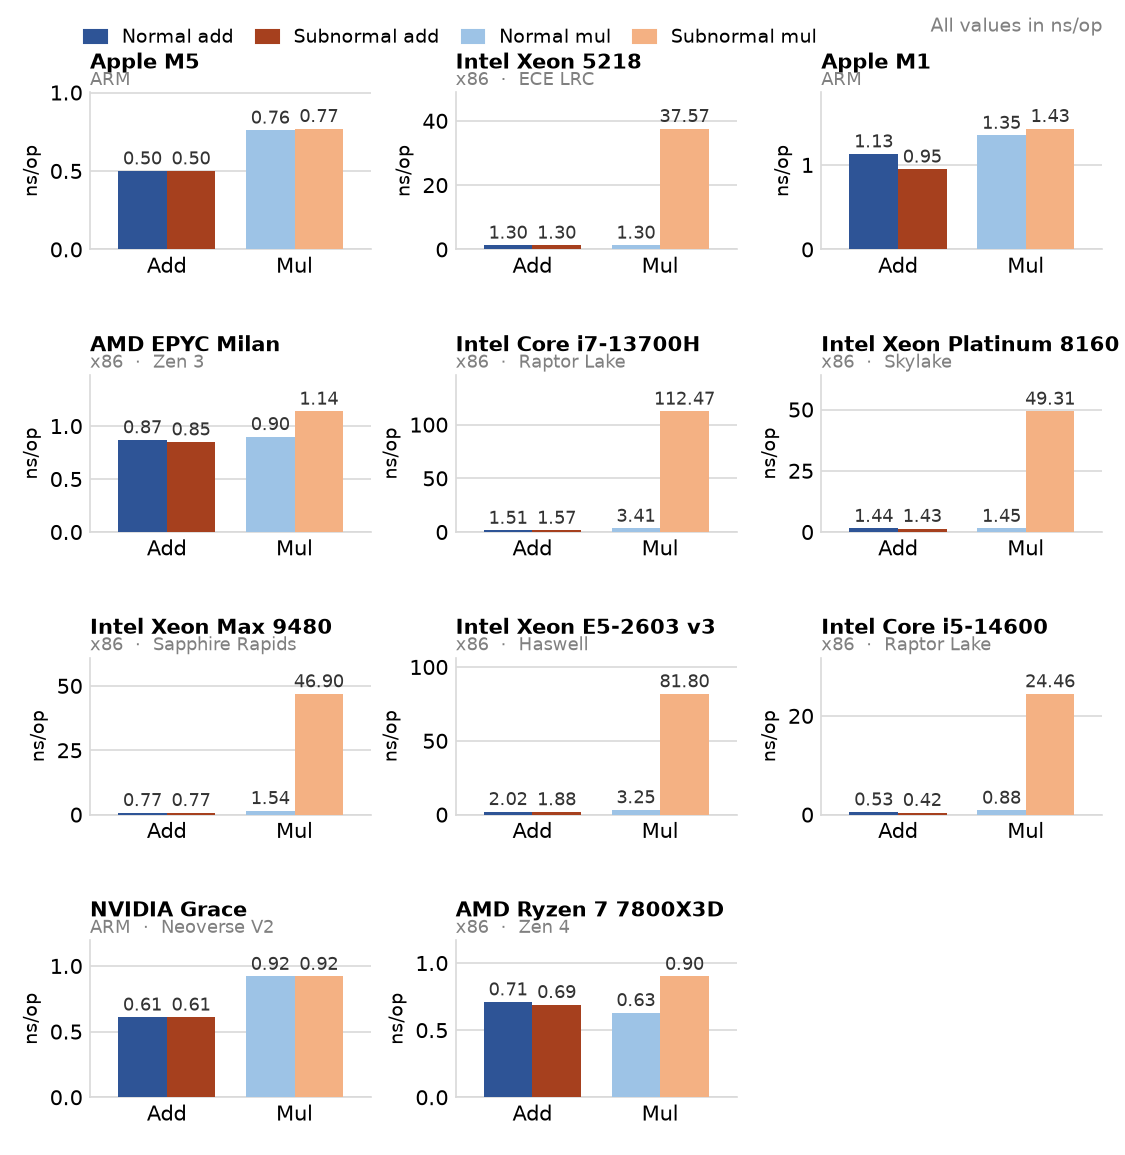
\includegraphics[width=\textwidth]{images/fp_timing_data.png}
    \caption{Time to perform floating-point instructions, measured in ns/op. Note the y-axis for each graph is different.}
    \label{fig:fp_timing_data} % Unique label used for referencing this figure
\end{figure*}

\subsection{Filter-Level Timing Gap}
\label{sec:filter_gap}
The data in Section~\ref{subsec:timing_data} times single instructions in a tight loop. To check that the gap also appears in the real filter computation, we wrote a small C program that runs the same math the SVG filter does (an \texttt{feColorMatrix} scale followed by repeated \texttt{feConvolveMatrix} passes), but outside the browser. It multiplies each pixel by a tiny factor $\alpha \approx 8.2\times10^{-42}$, which turns a white pixel (1.0) into a subnormal number and leaves a black pixel (0.0) at zero. It then runs 50 passes of a 25-tap averaging filter, about $10^{7}$ multiplications. We time an all-white buffer against an all-black buffer on the Intel Xeon 5218. White is about 16.5 times slower (50.2 vs.\ 3.0 ns per multiplication), matching the penalty from Section~\ref{subsec:timing_data}. Turning on Flush-to-Zero, which makes the hardware treat subnormals as zero, removes the gap (1.00 times) and drops the white result from a tiny nonzero value to exactly zero. This shows the slowdown comes from the subnormal values and nothing else.

This is the key piece the attack is built on: the filter's math is more than ten times slower on a white pixel than a black one. It does not yet mean the attack works in a browser, which must run the filter on the CPU rather than the GPU, keep the subnormals instead of flushing them to zero, and leave a timing gap big enough to see through browsers' coarse post-Spectre timers (Section~\ref{sec:attack_setup}). Testing that on the Xeon 5218 is our next step.

\subsection{The Attack Setup}
\label{sec:attack_setup}
We host a victim and an attacker website on separate local ports via a small Python server. The victim shows an 8x8 grid of 32 black and 32 white pixels in random order, fixed until the server restarts, which gives us a known ground truth to compare against.

The attack website loads the victim in a cross-origin iframe and confirms that the same-origin policy blocks it from reading the victim's DOM. It can then select a single pixel, enlarge it, and measure frame render times. Both calibration and scan modes work end to end, but since no SVG filter is applied yet, the frame times do not depend on pixel color and recover nothing.

One concern with the attack setup is timer precision. After Spectre, browsers reduced the precision of \texttt{performance.now()} and added jitter, and frame times are also limited by the display's refresh rate. We expect that we will need a large scale factor to make the subnormal penalty a large part of each frame's rendering time, and that we will need many samples per pixel to reliably tell the two colors apart.
